\section{SIMHYD (model ID: 18)}
The SIMHYD model (fig.~\ref{fig:18_schematic}) is a simplified version of MODHYDROLOG, originally developed for use in Australia \citep{Chiew2002}. It has 3 stores and 7 parameters (INSC, COEFF, SQ, SMSC, SUB, CRAK and K). The model aims to represent:

\begin{itemizecompact}
\item Interception by vegetation;
\item Infiltration and infiltration excess flow;
\item Preferential groundwater recharge, interflow and saturation excess flow;
\item Groundwater recharge resulting from filling up of soil moisture storage capacity;
\item Slow flow from groundwater.
\end{itemizecompact}

\subsection{MARRMoT model name}
m\_18\_simhyd\_7p\_3s \\

% Equations
\subsection{Model equations}

% Model layout figure
{ 																	% This ensures it doesn't warp text further down
\begin{wrapfigure}{l}{5cm}
\scalebox{0.7}{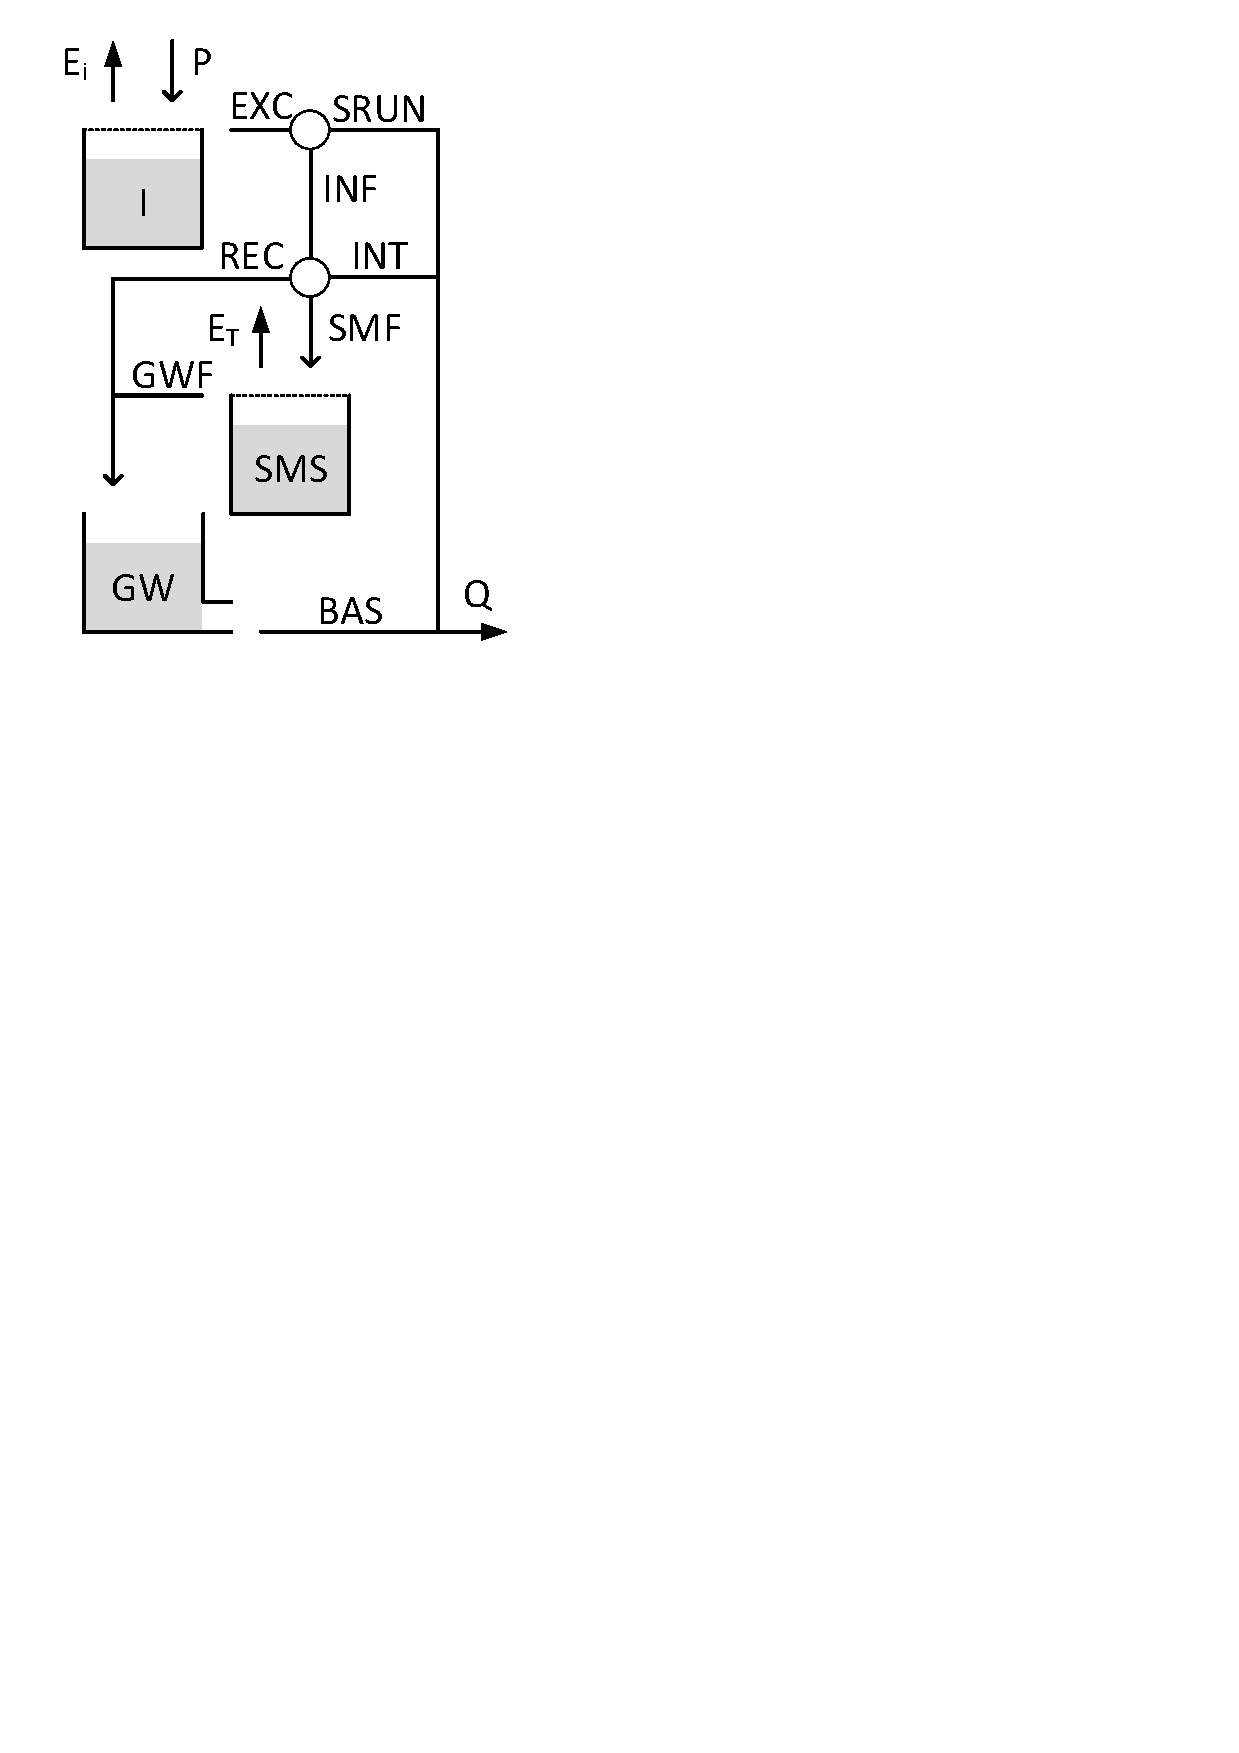
\includegraphics[trim=1cm 18cm 11.5cm 1cm,width=7cm,keepaspectratio]{./AppA_files/18_schematic.pdf}}
\caption{Structure of the SIMHYD model} \label{fig:18_schematic}
\end{wrapfigure}

\begin{align}
	\frac{dI}{dt} &= P-E_i-EXC \\
	E_i &= \begin{cases}
		E_p, &\text{if } I > 0 \\
		0, & \text{otherwise} \\
	\end{cases} \\
	EXC &= 
	\begin{cases}
		P, & \text{if } I = INSC \\
		0, & \text{otherwise}
	\end{cases}
\end{align}

Where I is the current interception storage [mm], $P$ precipitation [mm/d], $E_i$ the evaporation from the interception store [mm/d] and $EXC$ the excess rainfall [mm/d]). Evaporation is assumed to occur at the potential rate when possible. When I exceeds the maximum interception capacity $INSC$ [mm], water is routed to the rest of the model as excess precipitation $EXC$. 

} % end of wrapfigure
\vspace{1cm}
\begin{align}
	\frac{dSMS}{dt} &= SMF-E_T-GWF\\
	SMF &= INF-INT-REC\\
		&INF = min\left(COEFF * exp\left(\frac{-SQ*SMS}{SMSC}\right),EXC\right)\\
		&INT = SUB*\frac{SMS}{SMSC} * INF \\
		&REC = CRAK*\frac{SMS}{SMSC}*(INF-INT)\\
	E_T &=min\left(10*\frac{SMS}{SMSC},PET\right)\\
	GWF &= \begin{cases}
		SMF, &\text{if } SMS = SMSC\\
		0, &\text{otherwise}
	\end{cases}
\end{align}

Where SMS is the current storage in the soil moisture store [mm]. INF is total infiltration [mm/d] from excess precipitation, based on maximum infiltration loss parameter COEFF [mm/d], the infiltration loss exponent SQ [-] and the ratio between current soil moisture storage SMS and the maximum soil moisture capacity SMSC [mm]. INT represents interflow and saturation excess flow [mm/d], using a constant of proportionality SUB [-]. REC is preferential recharge of groundwater [mm/d] based on another constant of proportionality CRAK [-]. SMF is flow into soil moisture storage [mm/d]. $E_T$ evaporation from the soil moisture that occurs at the potential rate when possible [mm/d], and GWF the flow to the groundwater store [mm/d]:

\begin{align}
	\frac{dGW}{dt} &= REC+GWF - BAS\\
	BAS &= K * GW 
\end{align}

Where GW is the current storage [mm] in the groundwater reservoir. Outflow $BAS$ [mm/d] from the reservoir has a linear relation with storage through the linear recession parameter $K$ [$d^{-1}$]. Total outflow $Q_t$ [mm/d] is the sum of three parts:

\begin{align}
	Q_t &= SRUN+INT+BAS\\
	SRUN &= EXC-INF
\end{align}

\newpage
\subsection{Parameter overview}
% Table generated by Excel2LaTeX from sheet 'Sheet1'
\begin{table}[htbp]
  \centering
    \begin{tabular}{lll}
    \toprule
    Parameter & Unit  & Description \\
    \midrule
    INSC  & $mm$  & Maximum interception capacity \\
    COEFF & $mm~d^{-1}$ & Maximum infiltration loss \\
    SQ    & $-$   & Infiltration loss exponent \\
    SMSC  & $mm$  & Maximum soil moisture storage \\
    SUB   & $-$   & Proportionality constant \\
    CRAK  & $-$   & Proportionality constant \\
    K     & $d^{-1}$ & Runoff coefficient \\
    \bottomrule
    \end{tabular}%
  \label{tab:addlabel}%
\end{table}%



